\documentclass[a4paper, 11pt]{article}
\usepackage{AItemp}
\usepackage{epsfig,graphicx,subfigure,amsthm,amsmath, float, xcolor, changepage, mathtools, textcomp, hyperref, bm, amssymb, tcolorbox, tikz, setspace}
\usepackage[shortlabels]{enumitem}
\usepackage[stable]{footmisc}
\usepackage{xepersian}
\settextfont[Scale=1.2]{XBZar}
%\setdigitfont{XBZar}
\setlatintextfont[Scale=1.1]{Times New Roman}
\hypersetup{
	colorlinks=true,
	urlcolor=blue!70!black
}

\doublespacing
\begin{document}
\handout
{هوش مصنوعی}
{نیم‌سال اول ۰۱\lr{-}۰۰}
{دکتر محمدحسین رهبان}
{دانشکده مهندسی کامپیوتر}
{تمرین اول - بخش دوم}
{محمدجواد هزاره}
{98101074}
\noindent
\\ [-5em]
\section*{سوال ۱}
\begin{enumerate}[آ)]
	\item
	اگر در نظر بگیریم که در اجرای الگوریتم جست‌و‌جو با استفاده از 
	\lr{BFS}
	در لحظه‌ای که راسی به 
	\lr{fringe}
	اضافه می‌شود در همان لحظه تست هدف را اجرا کنیم، الگوریتم به صورت زیر اجرا می‌شود.	
	\begin{figure}[H]
		\centering
		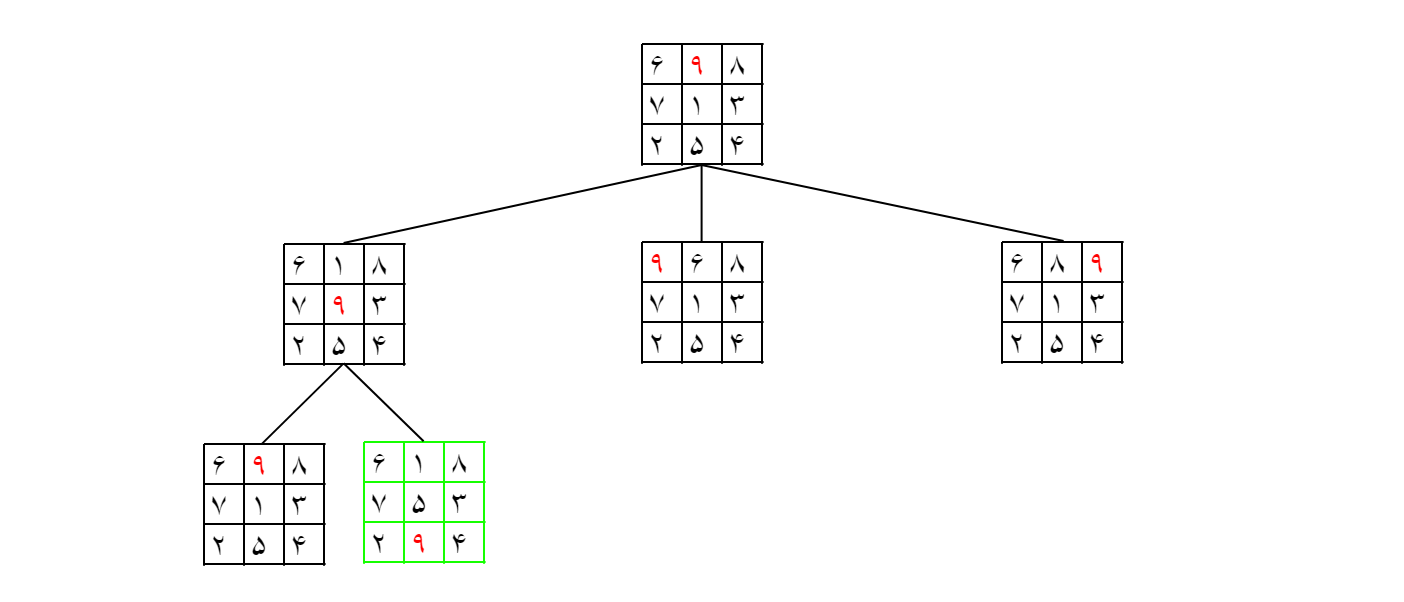
\includegraphics[width=\textwidth]{pics/tree-search.png}
		\caption{درخت جست‌و‌جو در روش درختی}
	\end{figure}
	پس از بررسی راس ریشه که حالت هدف نیست، نوبت به گسترش دادن این راس می‌رسد. برای گسترش دادن با الگوی (حرکت عدد ۹ به بالا، پایین، چپ و سپس راست) عمل می‌کنیم که در نتیجه راس سمت چپ از سطر دوم تولید می‌شود. در این روش به صورت خاص راس‌ها را در همان هنگام اضافه شدن به \lr{fringe} چک می‌کنیم، بنابراین این راس در همین مرحله چک شده و چون حالت هدف نیست به گسترش دادن ریشه ادامه می‌دهیم. دو راس دیگر این سطر نیز به ترتیب ساخته شده و بررسی می شوند که هیچ کدام حالت هدف نیستند. پس از این مرحله راس ریشه از \lr{fringe} خارج شده چرا که عملیات گسترش آن به پایان رسیده است و باید یک راس جدید از \lr{fringe} را برای گسترش انتخاب کنیم. این راس همان راس سمت چپ در سطر دوم خواهد بود چرا که ترتیب گسترش دادن نیز مشابه ترتیب تولید کردن راس‌هاست. با گسترش دادن این راس، اولین راس از سطر سوم تولید شده که این نیز شرط هدف را برآورده نمی‌کند. پس از آن راس دوم از سطر سوم تولید شده که شرایط مورد نظر مسئله را برآورده می‌کند و هدف است. بنابراین در این مرحله الگوریتم به پایان می‌رسد.
	\item
	در اجرا به صورت گرافی، راس‌هایی که حالت‌ آن‌ها را قبلا دیده‌ایم باز نمی‌کنیم. بنابراین درخت جست‌وجو پس از اجرای الگوریتم به صورت زیر باز خواهد شد.
	\begin{figure}[H]
		\centering
		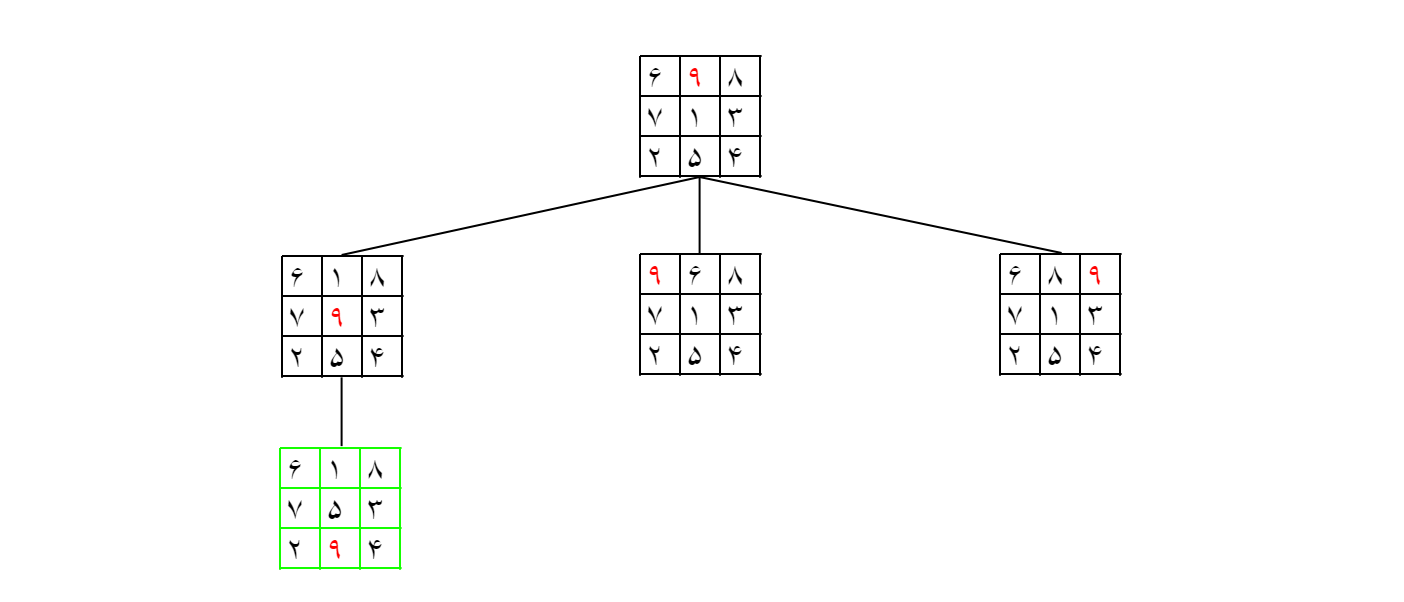
\includegraphics[width=\textwidth]{pics/graph-search.png}
		\caption{درخت جست‌وجو در روش گرافی}
	\end{figure}
	در این روش نیز به طور مشابه قسمت (آ) راس‌ها ساخته و بررسی می‌شوند. اما تفاوتی که در این‌جا وجود دارد آن است که در گسترش دادن راس سمت چپ در سطر دوم حالتی تولید می‌شود که الگوریتم قبلا آن را بررسی کرده است و همان حالت راس ریشه است. بنابراین این راس را تولید و بررسی نمی‌کنیم. پس از آن حالت بعدی که از پایین آوردن عدد ۹ بدست می‌آید تولید شده که هدف مسئله نیز هست و در این مرحله الگوریتم به پایان رسیده است.
	\item
	در مرحله اول روش \lr{IDS}، تا عمق صفر پیش می‌رویم که فقط شامل همان حالت اولیه می‌شود که شرایط هدف را برآورده نمی‌کند.
	\begin{figure}[H]
		\centering
		
\includegraphics[width=\textwidth]{pics/ids-1.png}
	\end{figure}
	در مرحله بعدی، 
	\lr{dfs}
	تا عمق یک داریم که درخت به صورت زیر باز می‌شود.
	\begin{figure}[H]
		\centering
		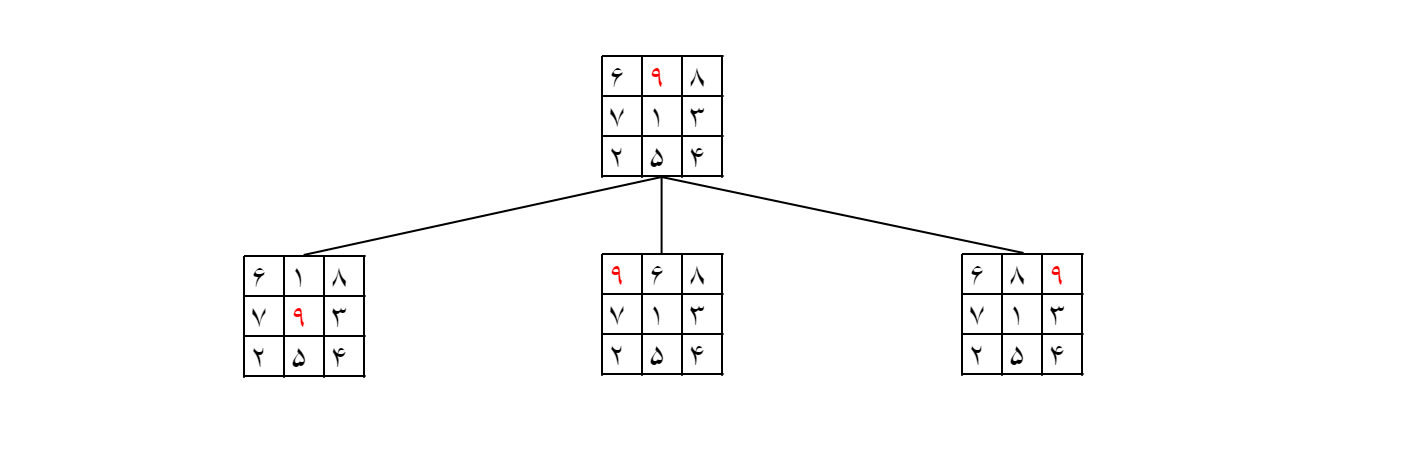
\includegraphics[width=\textwidth]{pics/ids-2.png}
	\end{figure}
	پس از این مرحله دوباره باید درخت را تا عمق دو جست‌وجو کنیم که در این مرحله به هدف می‌رسیم و از آن‌جایی که به صورت گرافی جست‌وجو کرده و از روش \lr{dfs} برای انتخاب راس‌های جدید از \lr{fringe} استفاده کرده‌ایم، درخت به صورت زیر باز می‌شود.
		\begin{figure}[H]
		\centering
		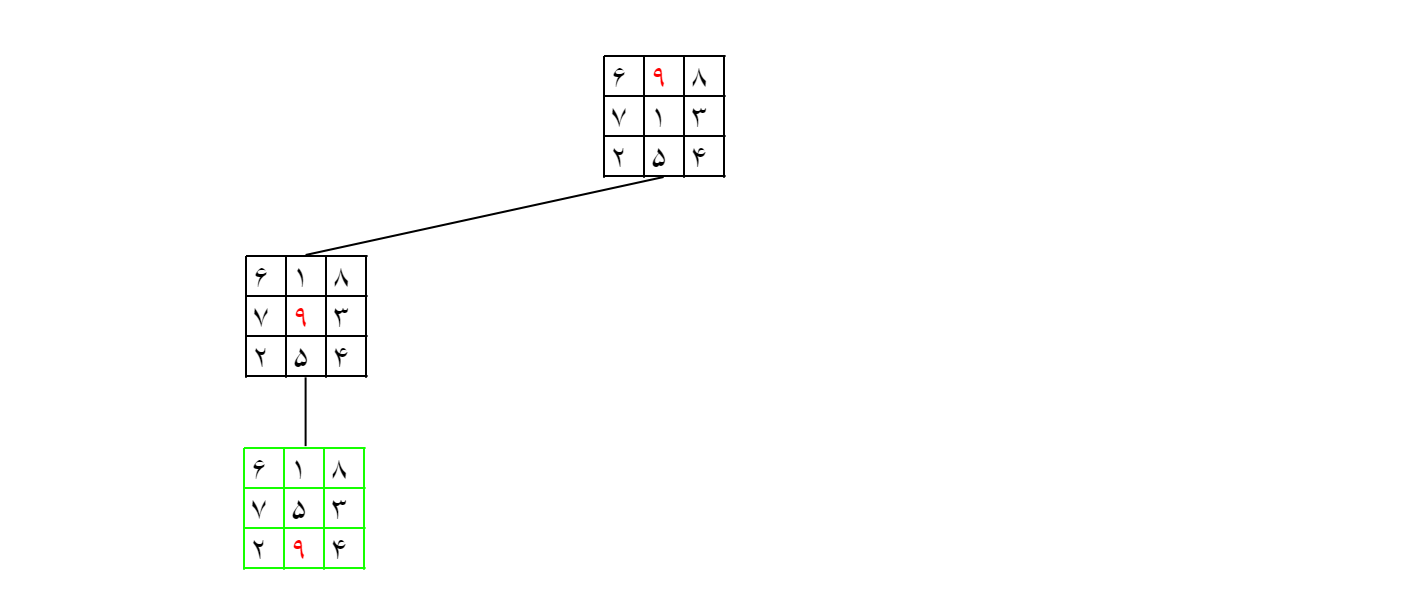
\includegraphics[width=\textwidth]{pics/ids-3.png}
	\end{figure}
\end{enumerate}

\section*{سوال ۲}
\begin{enumerate}[آ)]
	\item \textbf{درست است.}
	برای اثبات قابل قبول بودن
	$\bar{h} = max(0, \log_2 h(s))$
	، روی مقدار $h(s)$ حالت‌بندی می‌کنیم:
	\begin{itemize}
		\item $1 \le h(s)$:
		در این حالت لگاریتم $h(s)$ عددی نامنفی بوده و در نتیجه خواهیم داشت 
		$\bar{h} = \log_2 h(s)$.
		از طرفی چون خود $h(s)$ قابل ‌قبول است خواهیم داشت:
		\[
		\left.\begin{aligned}
			(\text{قابل قبول بودن $h(s)$}) &\quad h(s) \le h^*(s) \; \\
			(\log_2 x < x) &\quad \log_2 h(s) < h(s) \; \\
			&\quad \bar{h} = \log_2 h(s)
		\end{aligned}\right\}\implies \bar{h} < h^*(s)
		\]
		\item $0 \le h(s) < 1 $:
		در این حالت لگاریتم $h(s)$ عددی منفی بوده و در نتیجه مطابق تعریف داریم
		$\bar{h} = 0$.
		با توجه به قابل قبول بودن $h(s)$ و اینکه عددی بین ۰ و ۱ است داریم:
		\[
		\left.\begin{aligned}
			(\text{قابل قبول بودن $h(s)$}) &\quad h(s) \le h^*(s) \; \\
			(\text{فرض}) &\quad 0 \le h(s) \; \\
			&\quad \bar{h} = 0
		\end{aligned}\right\}\implies \bar{h} \le h^*(s)
		\]
	\end{itemize}
	بنابراین در هر حالت داریم 
	$\bar{h} \le h^*(s)$
	و این یعنی 
	$\bar{h}$
	قابل قبول است.
	\item \textbf{نادرست است!}
	مثلا تابع هیوریستیکی به صورت 
	$h(s) = h^*(s)$
	در نظر بگیریم، این تابع شرط قابل قبول بودن را داراست اما در راس‌هایی که هیوریستیک در آن‌ها مقداری بین 0 و 1 دارد، مقدار 
	$\sqrt{h(s)}$
	بزرگ‌تر از $h(s)$ و درنتیجه بزرگ‌تر از $h^*(s)$ خواهد بود که این شرط قابل قبول بودن را برای 
	$\sqrt{h(s)}$
	نقض می‌کند.
\end{enumerate}

\end{document}



